% !TEX root = ../../fyp.tex
\documentclass[../../fyp.tex]{subfiles}

\begin{document}
We carry out all experiments using GloVe word embeddings \cite{pennington} since all of the studies reproduced use some version of these and because these embeddings performed optimally in both \cite{moore2018} and \cite{bhuwandhingra2017} when dealing with NN based approaches. Since these word embeddings are case insensitive, we lowercase all tokens and carry out tokenization using the Spacy library with the default token filter (\S\ref{sec:filtering_embeddings}) to remove all emails and URLs from the text.

When determining parameters for each model, the following order is adopted; first, parameters from the original paper are set, while also referring to any accompanying source code which could include parameters missing from the papers. Where unavailable, we use configurations adopted by third-party implementations based on their reported results. Finally, we set any other parameters intuitively, based on the respective setting from models with similar architectures. 

As we shall outline, a non-trivial portion of the studies covered omitted essential parameter settings, such as the learning-rate of a model or the number of hidden units used, which drastically hinder their reproducibility. These omissions would be understandable provided the work is supplemented with source-code, however, this was also unobtainable or excluded in most cases.

Parameters such as the batch-size and duration of training are assumed based on online implementations, which report results similar to the original work. To account for this,following \cite{moore2018}, we adopt early-stopping with a patience of 10 epochs, a maximum allowance of 300 epochs and a minimum of 30 epochs, monitoring the loss metric of each model at every epoch. 

We first provide a brief overview of each approach, which is followed by a description of the challenges faced in reproducing each approach in particular, and the counter-measures taken. Finally, we contrast the results obtained from our experiments with those reported in the original work. Since he effect of the random seed on parameter initialization is statistically significant \cite{reimers2017} as cited in \cite{moore2018}, we report mean values from 3 separate runs using different random seed values, for each experiment. 

\subsection{TD-LSTM}
The work carried out by Tang et al 2016 was one of the first to employ LSTM based methods for the task of TSA. Three variants were developed for their experiments, first, a baseline LSTM model which did not take any target information into account. A Target Dependent(TD) LSTM integrated target information by concatenating the target vector to both left and right contexts, and using two separate LSTMs for each. Finally, a Target-Connected(TC) LSTM also adopted two LSTMs, however the target vector information was concatenated to each word in the context, rather than the context as a whole as in the TD-LSTM. This modification incurs a cost on computation time, as it effectively doubles the embedding dimension of each word. Each variant is followed by a softmax layer which is used to obtain the final classification of the sentence.  

The authors use the Dong et al. 2014 dataset, and experiment with both 100-dimension and 200-dimension twitter based GloVe embeddings. Furthermore, LSTM weights are initialized using U(-0.003,0.003) and training is carried out using stochastic gradient descent with a lerning rate of 0.01.

A notable omission in Tang et al. 2016 as well as the reproduction carried out by Moore  et al. 2018 is the hidden unit count for each LSTM cell. 

To choose a value for this parameter, experiments were carried out for each LSTM variant with 200 and 300 hidden units and both were found to converge on similar results. Since the latter requires more computational resources in training we assume a value of 200 for the results presented herein. 

The insignificant downstream differences between these two variants notwithstanding, the omission of this parameter makes reproduction attemps more challenging, and leaves room for uncertainty when comparing results to the original work. 

Finally, similar to Moore et al 2018, we ignore the reported 'softmax clipping threshold' of 200 as the implications of this remained misunderstood, and no further elaboration on the parameter is provided by Tang et al. 2016. 

As there was no mention of the batch-size or the amount of hidden units used in the kernel of the LSTMs these were set to be 200 and 64 respectively. These values were taken from online public implementations which quoted results similar to those reported in [Tang2016a]

Following on the approach by Moore, we vary the embeddings being used in termed of dimensionality so as to test the observed improvement in results with its increase. 

We also increase the upper bound to 300d by including the two variants of the glove embeddings which are sourced from a wider vocabulary, not exclusive to twitter, which could make them better suited for the restaurants and laptops datasets. 

Finally, the larger of these two variants also takes into account another aspect by differentiating between uppercase and lowercase letters in tokens. 

We consider the performance of the TD-LSTM as it is the most commonly quoted variant compared in the literature. 

Comparing macro-f1 scores to account for the class imbalances in each dataset we note that the 300d GloVe variants outperform the 100d and 200d embeddings, even though the latter are not sourced from twitter as is the dataset. The 840b variant obtains the best score, suggesting that there is valuable information contained in the case-sensitivity of tokens.


When considering the laptops and restaurants dataset, which differ to dong in terms of class balance and sample length [REF Chapter on datasets], performance drops significantly. 

Although the non-twitter embedding variants slightly outperform their counterparts in the laptop dataset, the best mean result is 56.55\% indicating the model's poor capacity for learing from the dataset. 

The same can be said for the restaurants dataset, considering the wide variance in the results observed using any embedding with the best results being counterintuitively obtained by the 100d twitter-sourced glove variant.

When considering the results obtained for the Dong dataset, we note that both 100d and 200d glove embeddings perform similarly, with a slight edge in the mean of the 200d variant. This notwithstanding, both variants' performance is markedly less than that reported in the original paper [Tang], which as stated in [Moore], can be attributed reporting only results from singular runs, thus not taking into account the downstream effects of differences in random initializations of weights. 

Finally, the performance of the 300d embedding variants in comparison, is in accordance with the upward trend with increased dimensionality noted in [Moore]

When comparing the results obtained in the laptops and restaurants dataset to those reported in [Chen2017] there is a significant difference irrespective of the embedding used. Although this can also be caused by randomness in the wegiht initializations (no mention of multiple runs is made), it is interesting to note that the opposite phenomena is observed when considering the dong dataset. In this instance the result reported by [Chen2017] is substantially lower than the rest.

This discrepency may be the result of the different approaches that were adopted to account for unknown parameters in the original work [Tang2016a] which were similarly left unreported in [Chen2017].


\begin{figure}[!ht]
	\centering
	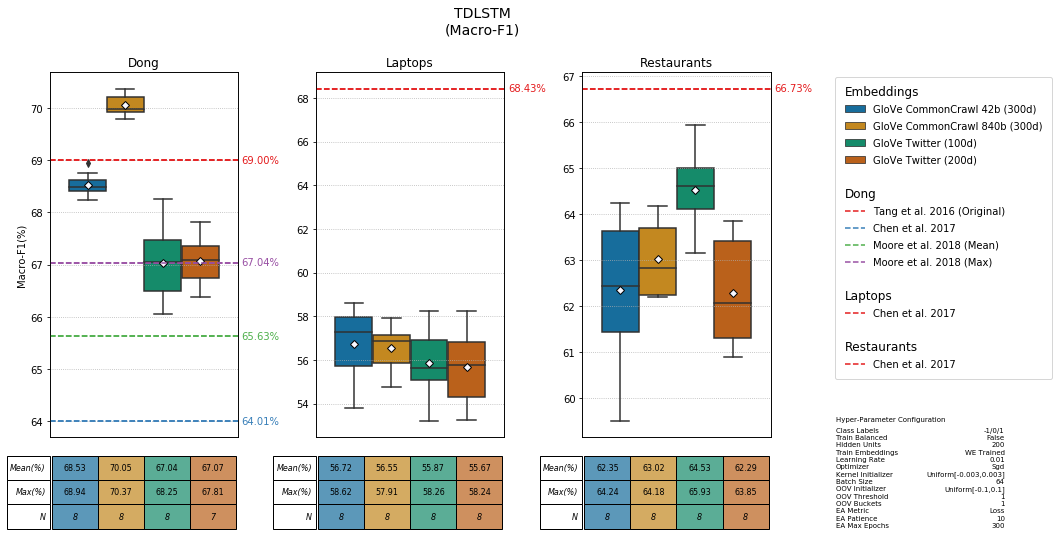
\includegraphics[width=\textwidth]{tdlstm_orig_macrof1.png}
	\caption{TD-LSTM Macro-F1 Results, $N$ refers to the number of runs carried out.}
	\label{fig:ffnn}
\end{figure}

\end{document}